
\section{Android App Prototype}

The prototype Android app, developed for this paper, is a simple weather app. It is able to show the current weather data for a location including temperature, humidity and wind. For retrieving this data, the app connects to the remote \emph{application programming interface} (API) of \emph{openweathermap.org}, a free-to-use service for retrieving weather data. The app also manages a list of favourite locations. Locations can either be specified using a free-text search field or by pointing locations on a map, for which the \emph{Google Maps} API was used.

\subsection{App Structure}

As mentioned above, the basic building blocks of an Android application are \emph{Activities} and \emph{Fragments}. Applying MVP to an Android application therefore means to put attention on those components.

The implementation of MVP in the app prototype, follows the approach of Leiva \cite{AntLeiv14}, in which \emph{Activities} implement the view part. This means that in addition to extending the base Android \texttt{Activity} class, an activity class must also implement a \texttt{View} interface. The class structure around such an activity is illustrated in Fig. \ref{fig:androidmvp}.

\begin{figure}[h]
\centering
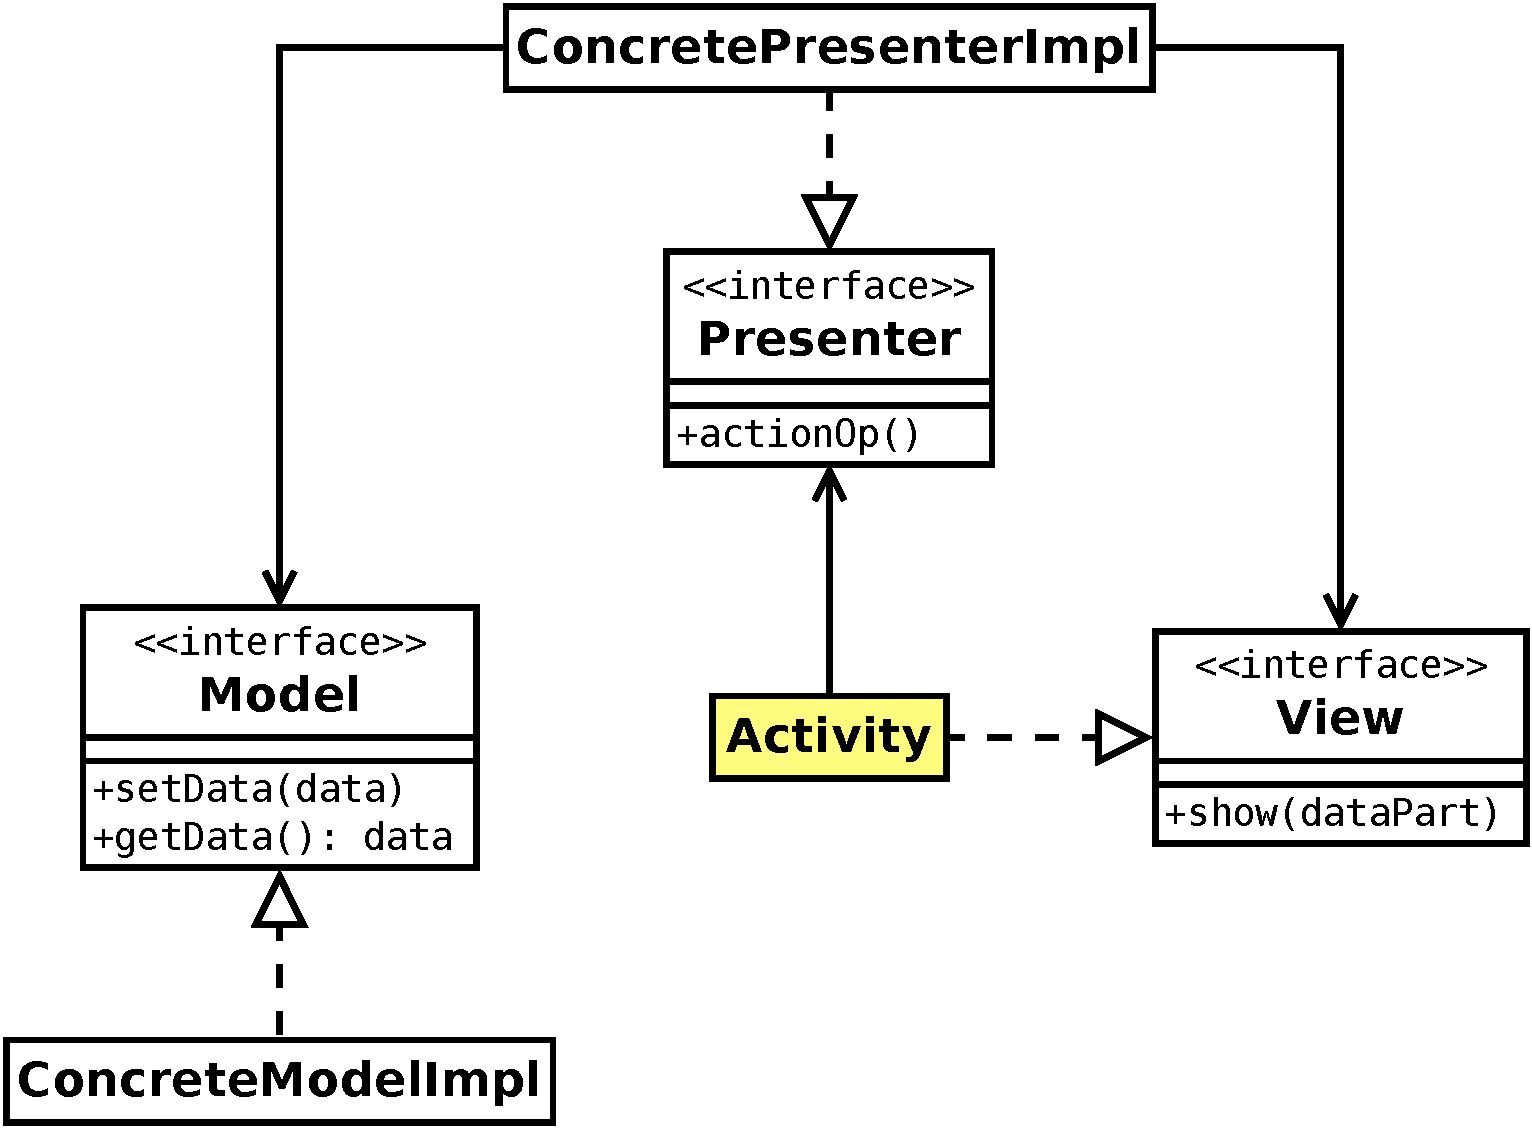
\includegraphics[width=0.45\textwidth]{diag1.pdf}
\caption{Class structure of an activity (highlighted with yellow background) in the context of an MVP architecture}
\label{fig:androidmvp}
\end{figure}

Each activity object has an presenter object associated, implementing the \texttt{Presenter} interface. On the other hand, the presenter object has a reference to the activity object. View related actions, like a click on a button, cause handler functions inside the \texttt{Activity} class being called. Those handler functions do nothing more than executing corresponding actions on the presenter object.

The interaction with the model is done only by the presenter. This makes the app prototype an implementation of the \emph{Passive View} kind of MVP.
An example of an interaction sequence between objects of \texttt{Activity}, \texttt{Presenter} and \texttt{Model} classes is shown in Fig. \ref{fig:androidmvpseq}. Clicking on a button -- let's assume it's labeled \emph{Refresh} -- causes the handler function in the \texttt{Activity} being called. An action is executed on the presenter object by the activity. The presenter retrieves new data from the model and afterwards calls the activity (the \texttt{View}) for showing that data.

\begin{figure}[h]
\centering
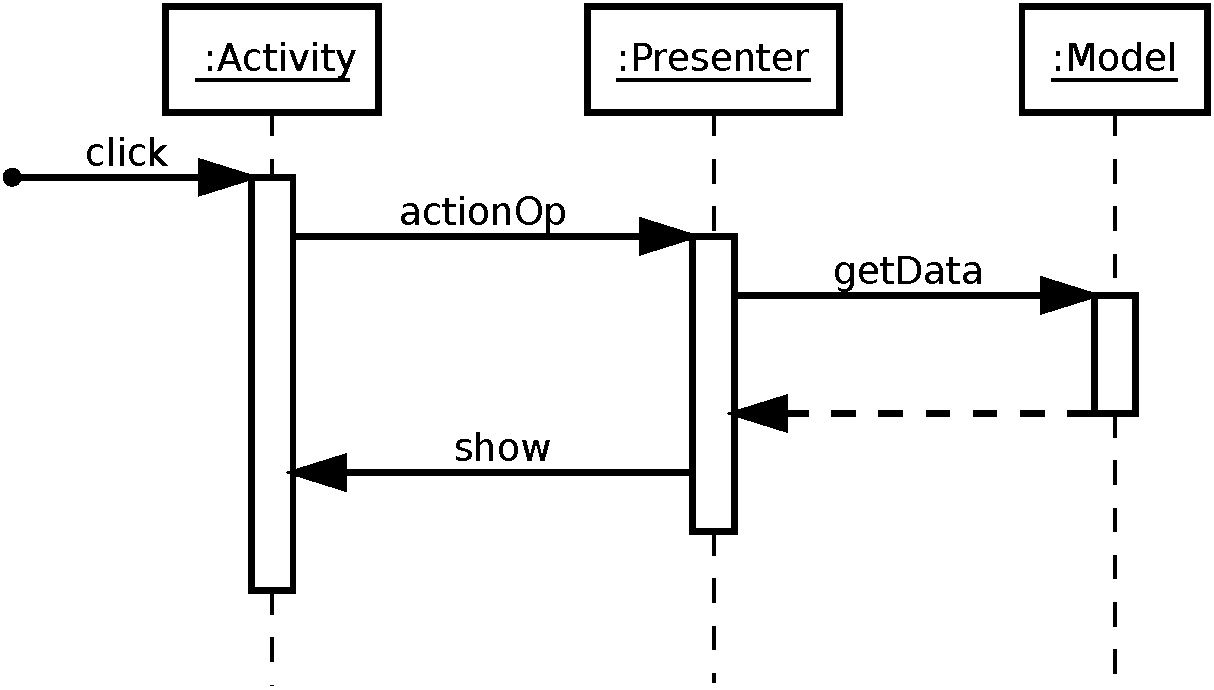
\includegraphics[width=0.45\textwidth]{diag2.pdf}
\caption{Interaction sequence involving objects of \texttt{Activity}, \texttt{Presenter} and \texttt{Model} classes}
\label{fig:androidmvpseq}
\end{figure}

For model operations that take a while to execute -- like retrieving weather data from \emph{openweathermap.org}, which can take a few seconds -- the interaction between presenter and model was implemented in an asynchronous way. Model objects, used by multiple presenters, additionally implement the \emph{Observer} design pattern (see \cite[p. 287]{GangOfFour}) to notify all registered presenters on model changes.

The MVP pattern can be applied to \emph{Fragments} the same way as it is described above for \emph{Activities}. Presenters of \emph{Fragment} objects most likely share their model with other \emph{Fragments} and other \emph{Activities}. An example of this was implemented in the \texttt{WeatherDetailsActivity} of the app prototype, which shows the weather data for a selected location. The part of the view showing temperature and wind information was extracted into a separate \emph{Fragment} with its own presenter implementation. Clicking on the \emph{Refresh} button causes the presenter of the activity to instruct the model to fetch updated weather data from \emph{openweathermap.org}. When this data is available, the model notifies all registered observers -- in this case the presenter of the activity and the presenter of the fragment. Both presenters go back to the corresponding view objects and cause the updated data to be displayed.

\todo[inline]{Maybe add something about Intents here}

This answers RQ3, showing that MVP can be applied to an Android application considering the \emph{Activity} and \emph{Fragment} building blocks.

As an additional remark, the usage of the \emph{Dependency Injection} (see \cite{FowlerIoC}) library \emph{Dagger} should be mentioned. The library was used to resolve object dependencies, like the one which exists between an \texttt{Activity} and an \texttt{Presenter} object (and vice versa). It automatically injects references of both objects into each other.

\subsection{Testing the App}

As mentioned before in section \ref{sec:research}, a key benefit of an MVP architecture is the increased testability of the software.
To demonstrate this ability, some tests for the app prototype were created using the testing capabilities of the Android SDK -- the Android testing framework:

\textbf{Activity Unit Test}:
An activity object will be created in an isolated environment. This means that, except from the tested activity object, every other component, like the application itself, is replaced by a mock implementation. This includes the presenter object as well. Using such a mock presenter implementation allows to easily test the interaction between an activity and its presenter.
An example would be the simulation of a button click and the assertion, if the presenter object was called correctly.
Without having MVP in place, the isolation of an activity object would be way more complicated or may even not be possible at all.

\textbf{Model Unit Test}
As the model objects of the app prototype have no dependency to any Android related component, they are very good for being tested through unit tests. As described for activities above, the model object will be created in an isolated environment with a mock presenter implementation.
